\documentclass{article}
\usepackage{listings}
\usepackage{verbatim}
\lstset{
    frame=single,
    breaklines=true
}
\usepackage{geometry}
\geometry{margin=1in}		%set margins

\usepackage{graphicx}		%need for images
\usepackage{float}			%need for arranging graphics and tables


\title{ECG 782 HW 4}
\date{2015-10-15}
\author{Carlo Lopez-Tello}

\begin{comment}

how to paste code

\lstinputlisting[language=Octave]{Q1/histEqualize.m}

how to paste image

\begin{figure}[H]
	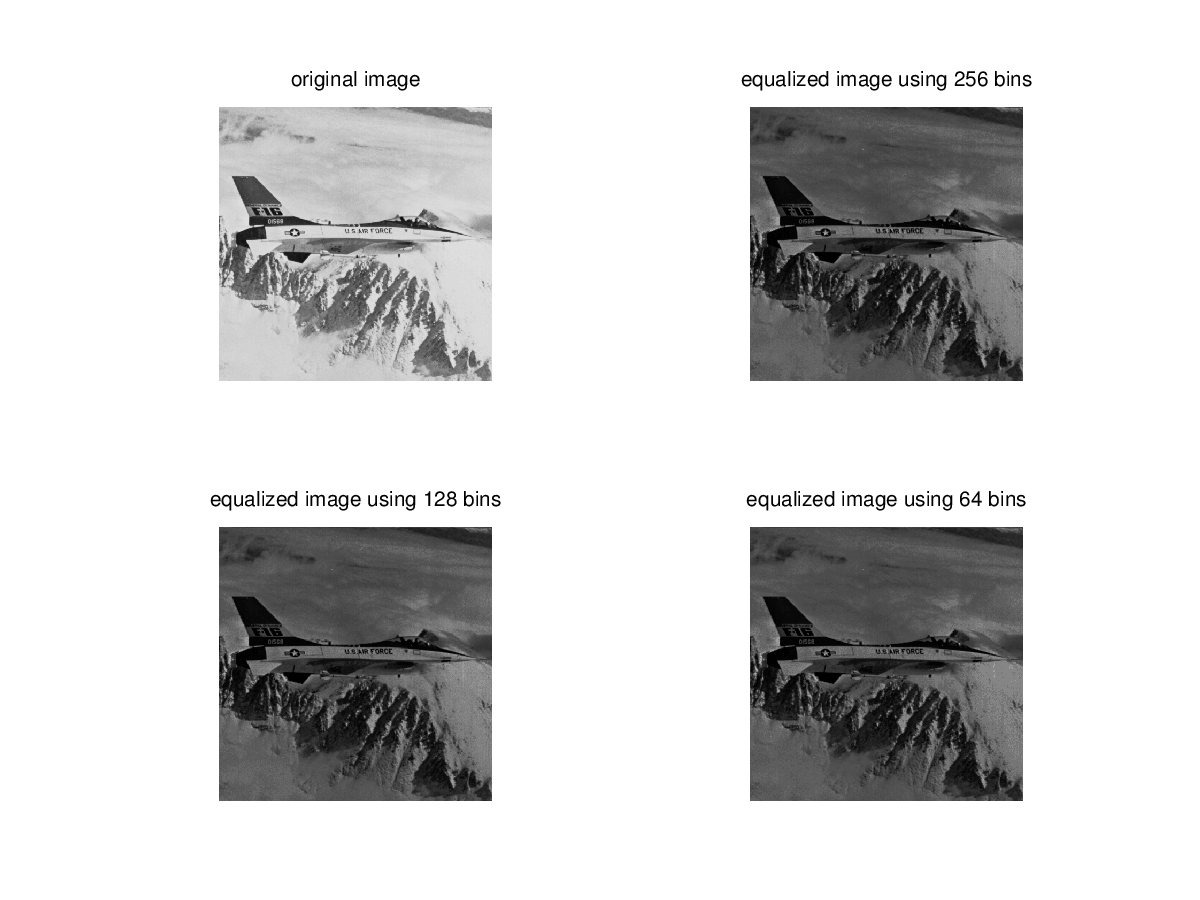
\includegraphics[width=\linewidth]{Q1/outputImages.png}
	\caption{equalized images}
\end{figure}

how to start newpage

\newpage

how to make table

\begin{table}[H]
	\centering
	\begin{tabular}{ c | c | c }
		filter & MSE & PSNR \\
		none & 72.0 & 29.6 \\
		3x3 mean filter & 32.9 & 33.0 \\
		5x5 mean filter & 36.7 & 32.5 \\
		3x3 median filter & 37.2 & 32.4 \\
		5x5 median filter & 36.2 & 32.5 \\
	\end{tabular}
	\caption{SNR and PSNR after filtering the noisy image}
\end{table}
	

\end{comment}
\begin{document}
\maketitle
	\newpage
	\section{Problem 10.6}
	
	\begin{figure}[H]
		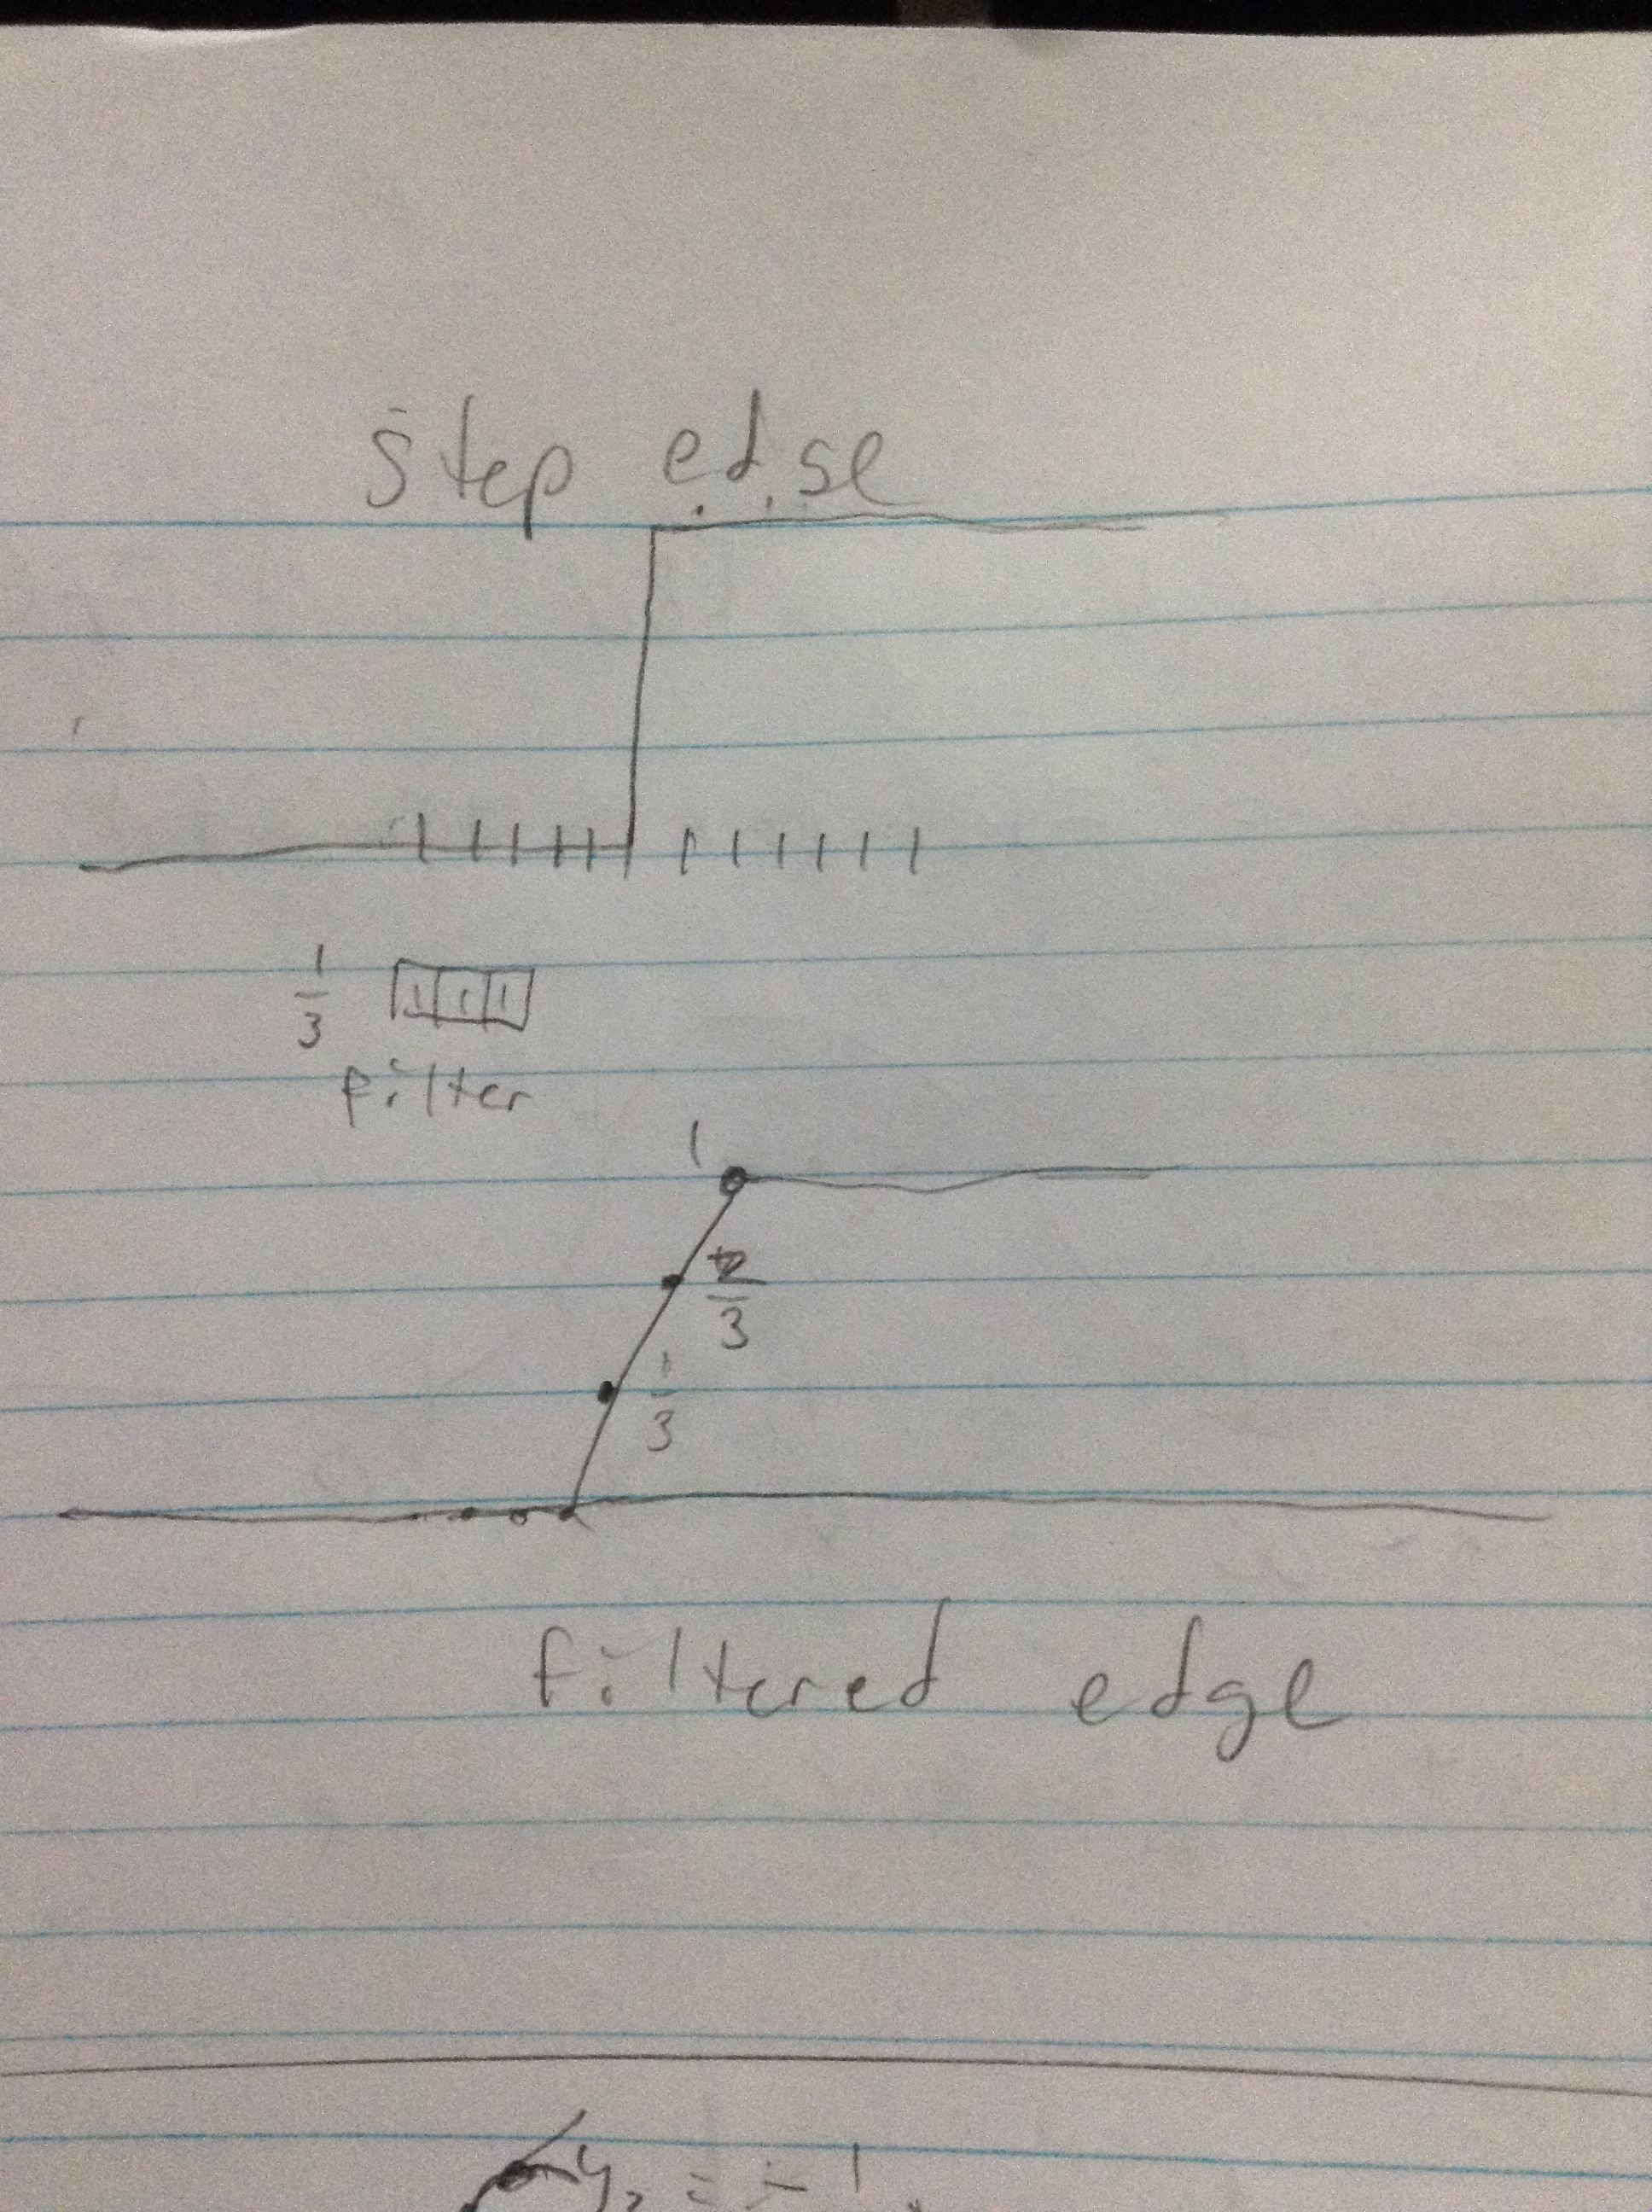
\includegraphics[width=\linewidth]{fig2.JPG}
	\end{figure}
	
	\newpage
	\section{Problem 10.22}
	\begin{figure}[H]
		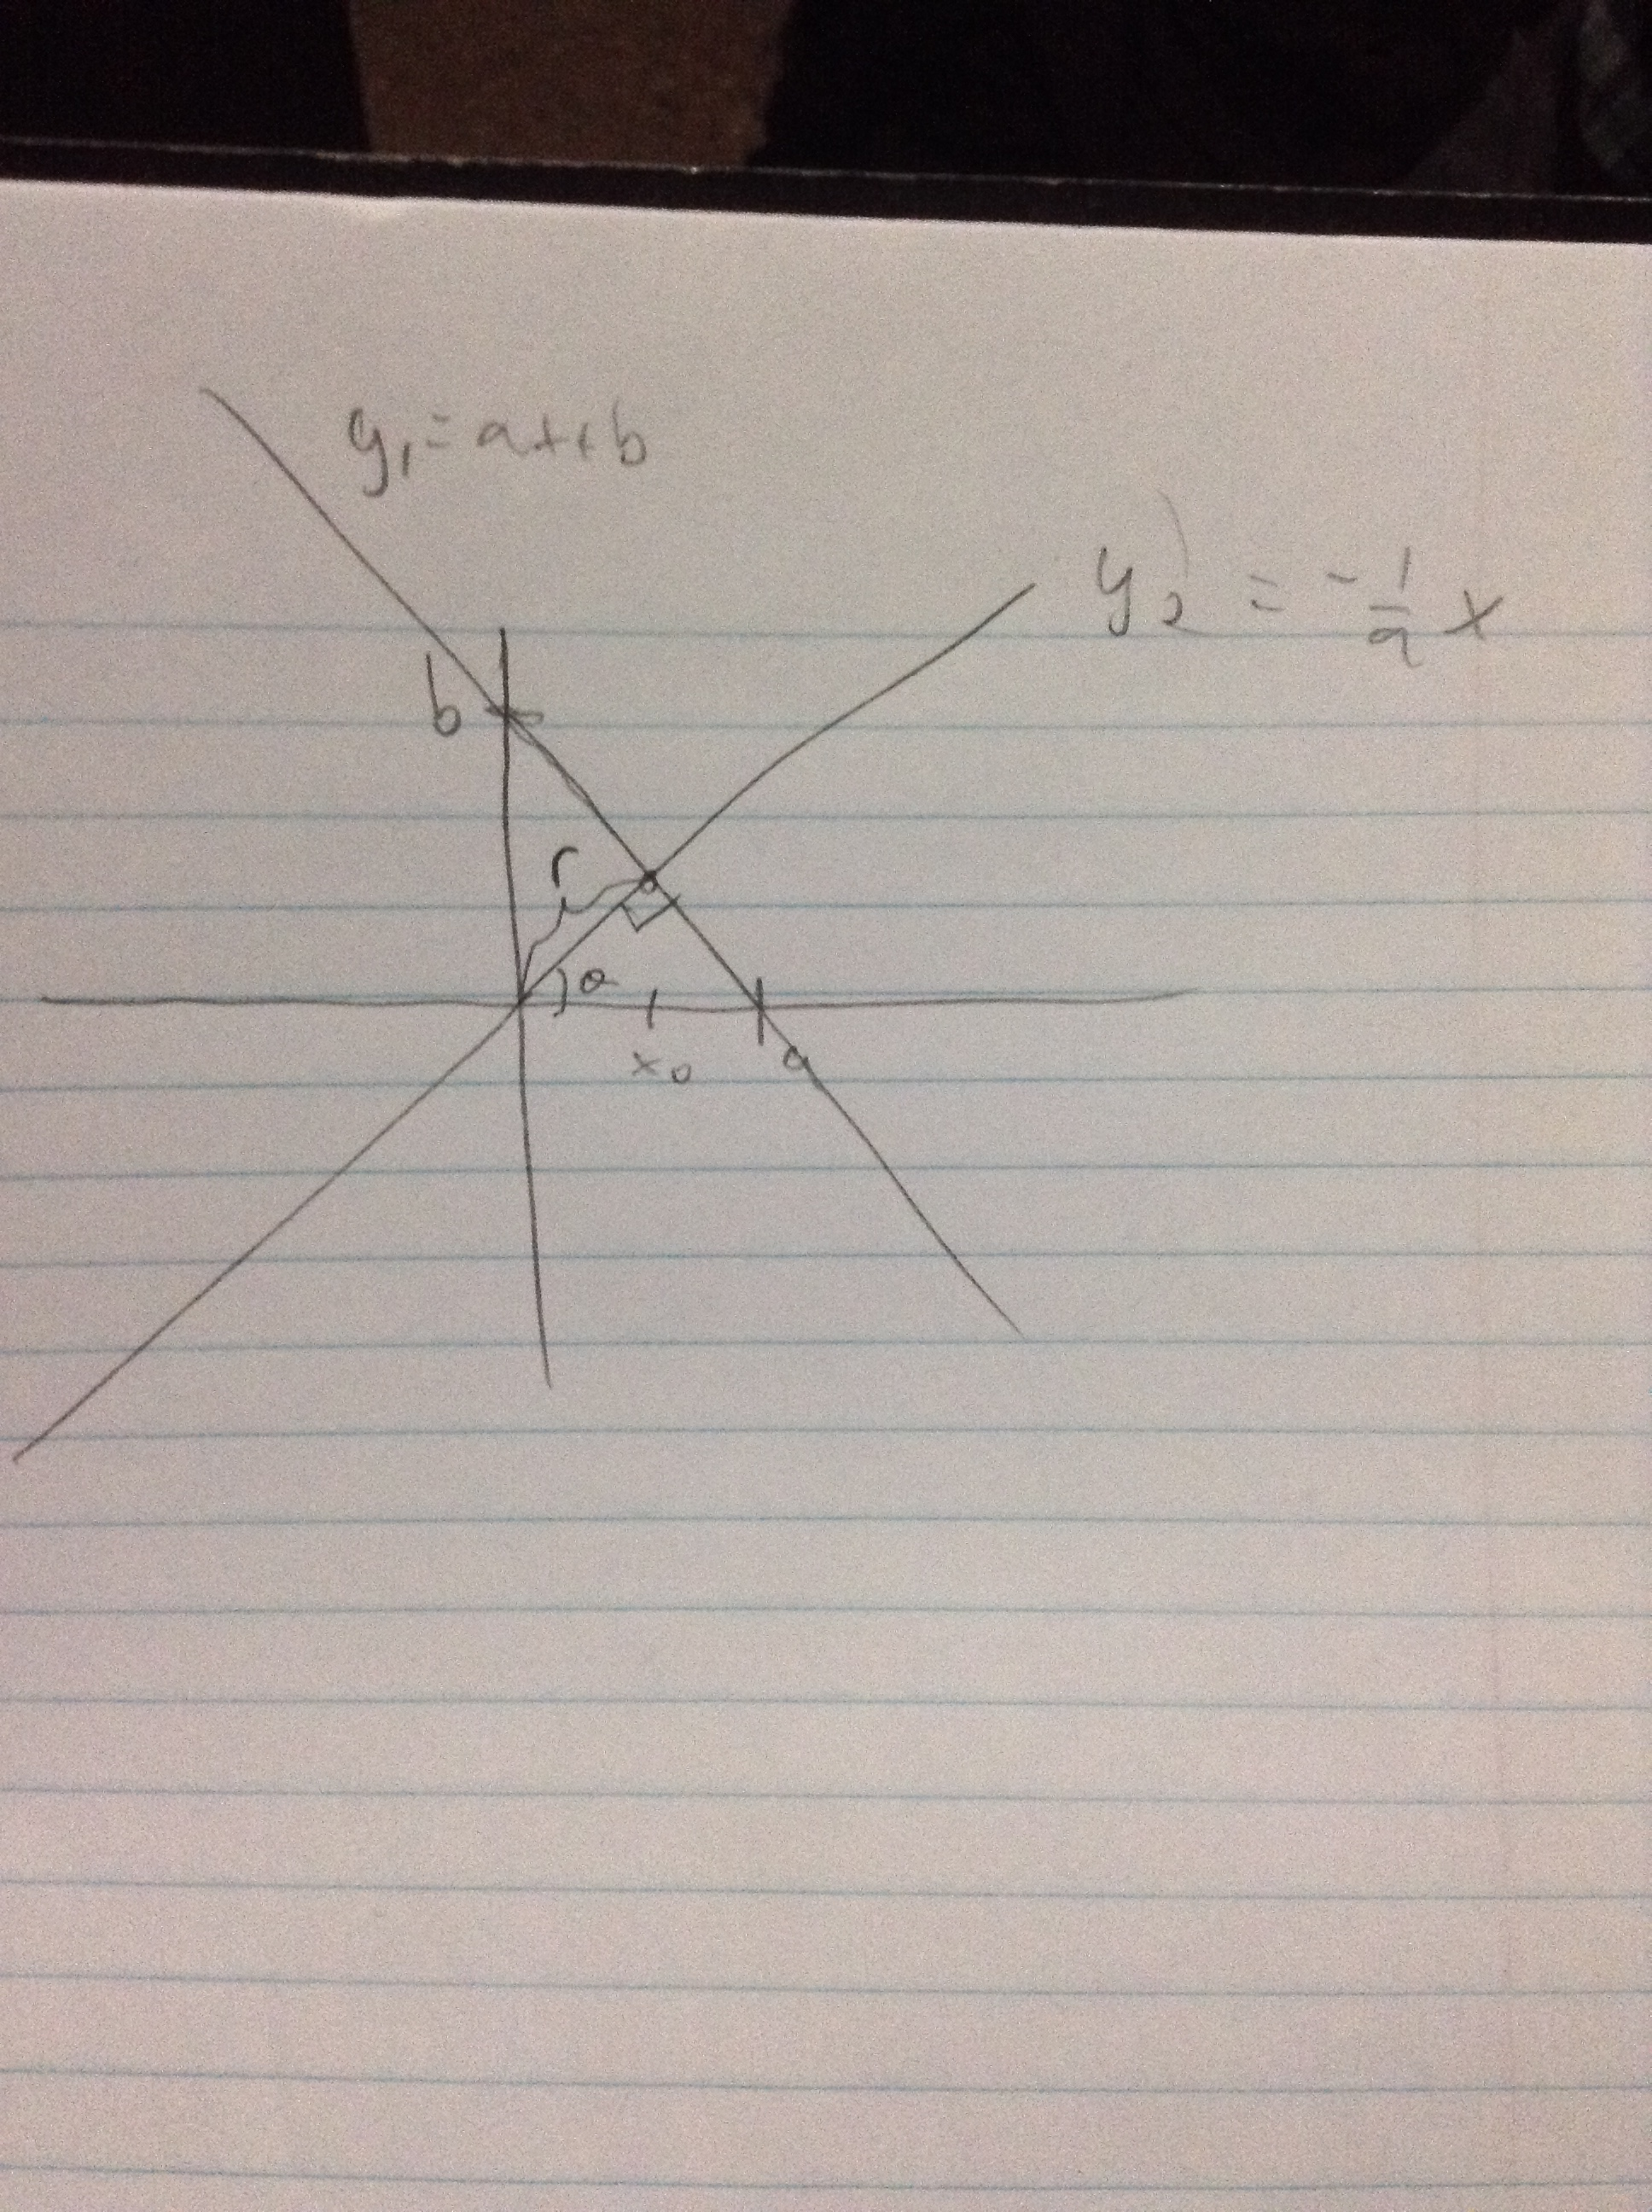
\includegraphics[width=\linewidth]{fig3.JPG}
	\end{figure}
	
	The slope of \(y_2 = -\frac{1}{a}x\). This implies that \(\theta = atan(-\frac{1}{a})\).
	We can find \(x_0\) by solving the following equation.
	\[y_1 = y_2\]
	\[ax + b = -\frac{1}{a}x\]
	\[b = -\frac{1}{a}x - ax\]
	\[b = (\frac{1}{a} + a)-x\]
	\[-b = (\frac{1}{a} + a)x\]
	\[-\frac{b}{(\frac{1}{a} + a)} = x\]
	\[x_0 = x\]
	\[x_0 = -\frac{b}{(\frac{1}{a} + a)} \]
	We can find r by solving the following equation.
	\[rcos(\theta) = x_0\]
	\[r = \frac{x_0}{cos(\theta)}\]
	\[r = \frac{-\frac{b}{(\frac{1}{a} + a)} }{cos(atan(-\frac{1}{a}))}\]
	
	
	If \(y = -3x + 2\) then \(a = -3\) and \(b = 2\) 
	\[\theta = atan(-\frac{1}{a}) = atan(-\frac{1}{-3}) = 18.4^\circ)\]
	\[x_0 = -\frac{b}{(\frac{1}{a} + a)} = -\frac{2}{(\frac{1}{-3} + -3)} = .6\]
	\[r = \frac{x_0}{cos(\theta)} = \frac{.6}{cos(18.4^\circ)} = \frac{.6}{.95} = .63\]
	
	
	\newpage
	\section{Problem 10.36}
	
	\begin{figure}[H]
		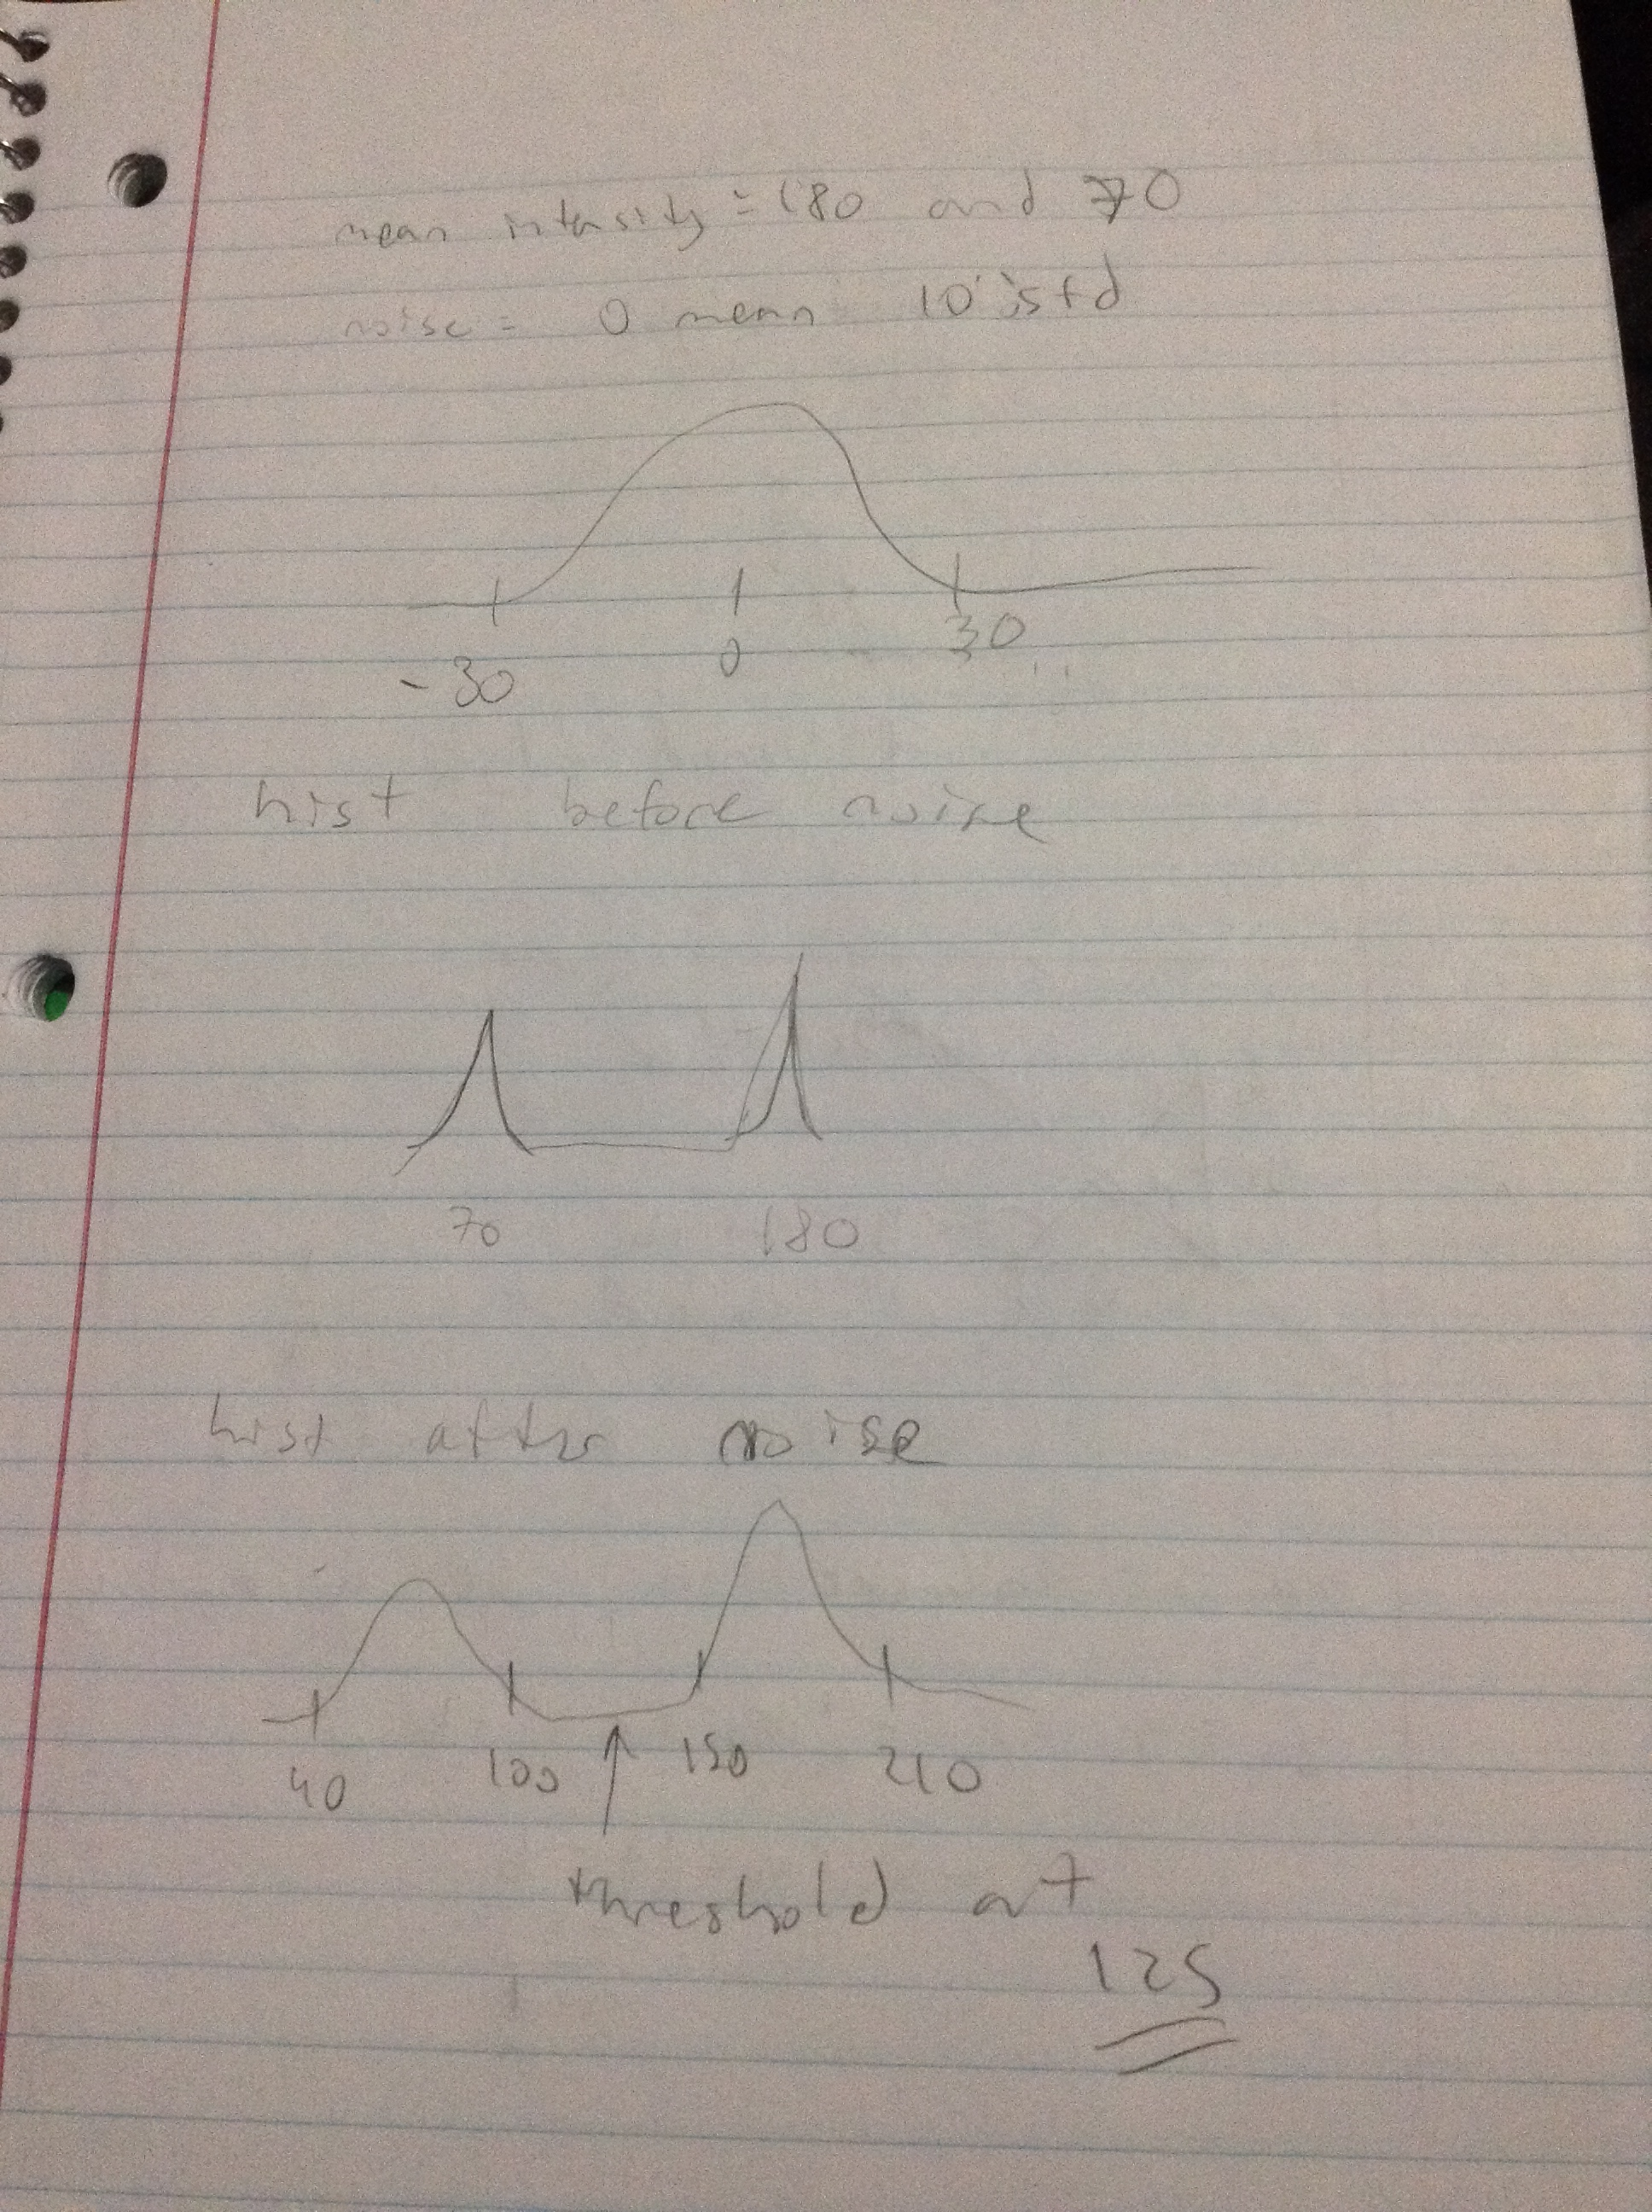
\includegraphics[width=\linewidth]{fig1.JPG}
	\end{figure}
	
	\newpage
	\section{Problem 4}
	
	The error for a given T threshold value can be obtained from the following:
	\[ E(T) = P_1\int_{T}^{\infty}p_1(z) + P_2\int_{-\infty}^{T}p_2(z) \]
	\[ \frac{d}{dt}E(T) = -P_1p_1(T) + P_2p_2(T) \]
	\[ 0 = -P_1p_1(T) +  P_2p_2(T) \]
	\[ P_1p_1(T) = P_2p_2(T) \]
	Since \( P_2 = P_1 \)
	\[ p_1(T) = p_2(T) \]
	\[ 1 - .5T = -.5 + .5T \]
	\[ 1.5 = T \]
	
	\newpage
	\section{Problem 5}
	\subsection{Gradient Kernel}
	\begin{figure}[H]
		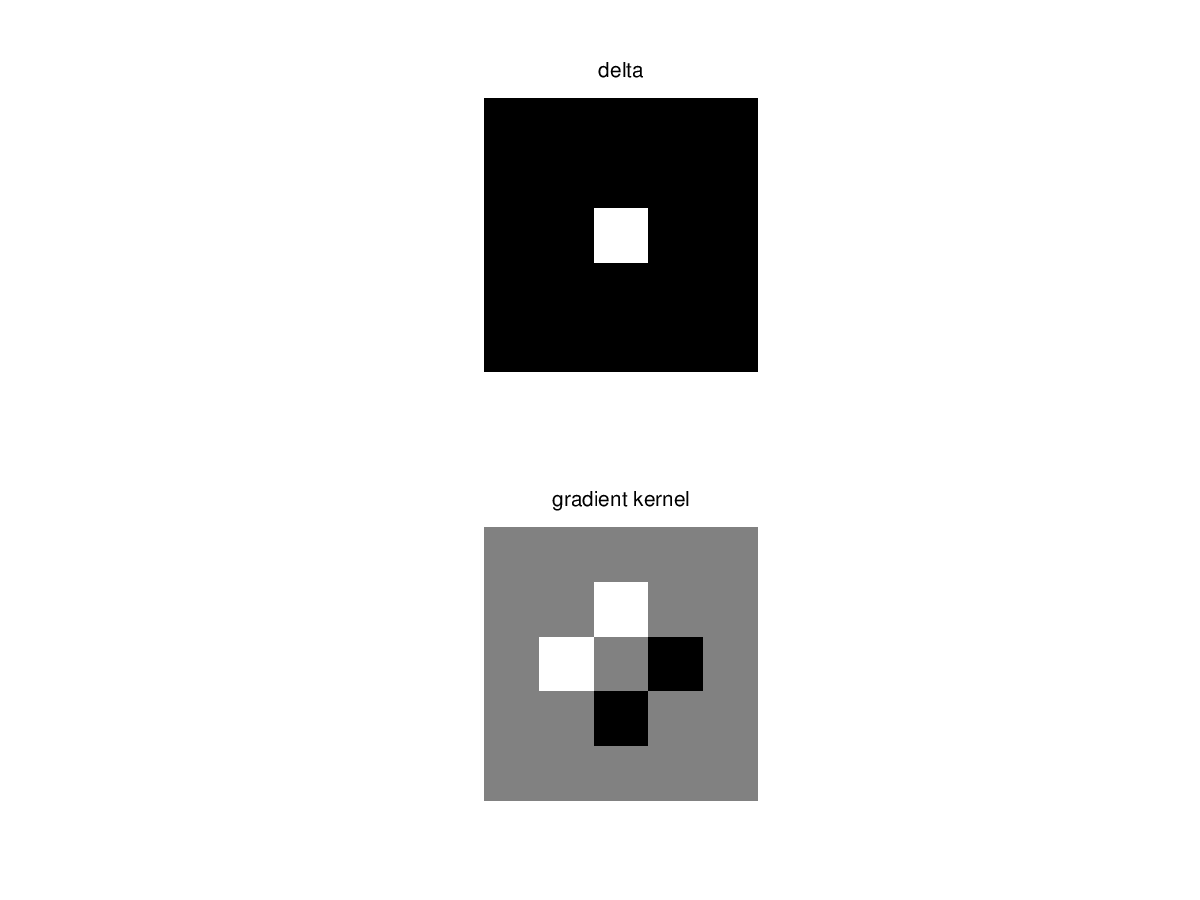
\includegraphics[width=\linewidth]{Q5/partA.png}
	\end{figure}
	The kernel used is [.5 0 -.5] in each direction.
	
	\newpage
	\subsection{Implement a simple version of the Canny edge detector}
	\lstinputlisting[language=Octave]{Q5/canny.m}
	
	\newpage
	\subsection{Apply the canny edge detector to wirebondmask.tif}
	\begin{figure}[H]
		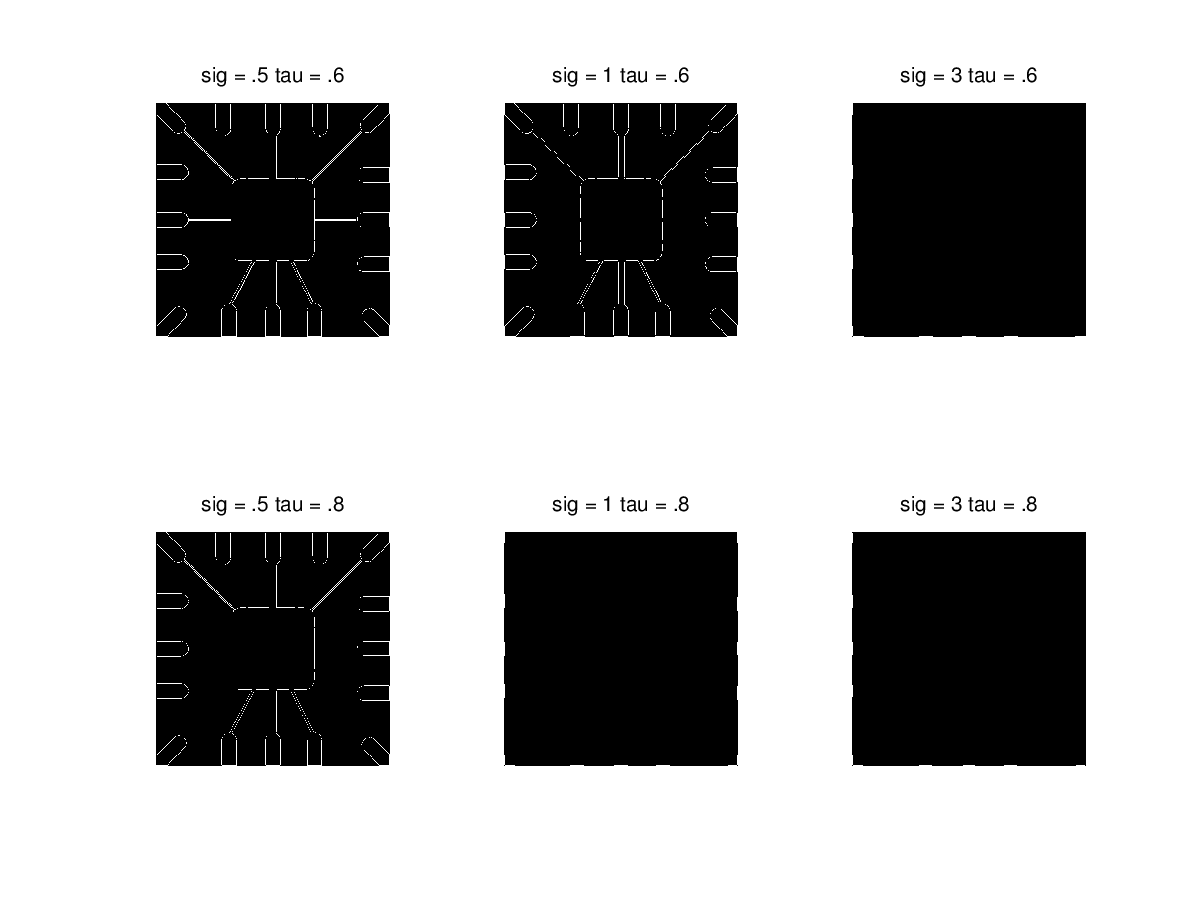
\includegraphics[width=\linewidth]{Q5/partC.png}
	\end{figure}
	Applying bigger filters to smooth the image before edge detection appears to decrease the intensity of the edges. This can be seen by the smaller amount of edges that are visible when using the same threshold value. This problem appears to be caused by border artifacts in the images. 
	
	
	\newpage
	\subsection{Apply the canny edge detector to city.jpg}
	\begin{figure}[H]
		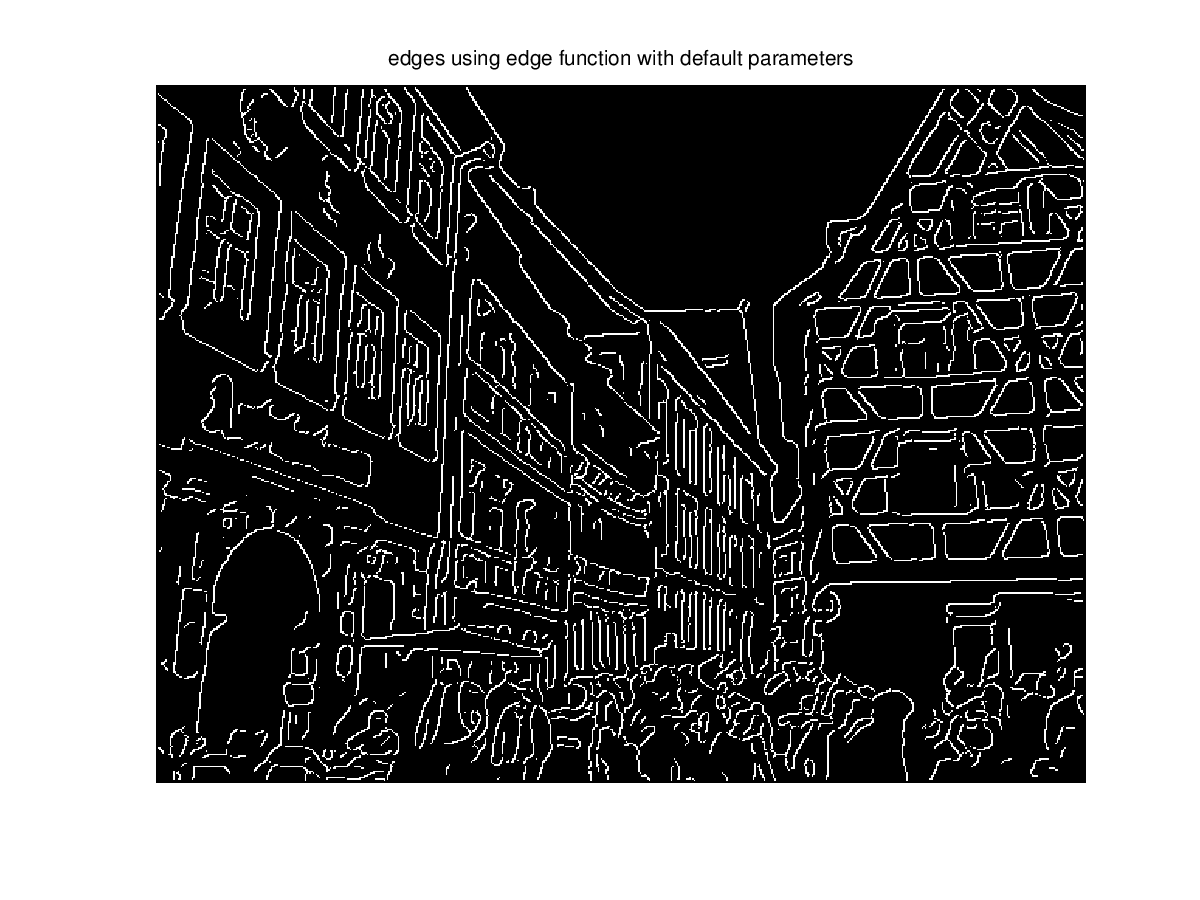
\includegraphics[width=\linewidth]{Q5/partD1.png}
	\end{figure}
	
	\begin{figure}[H]
		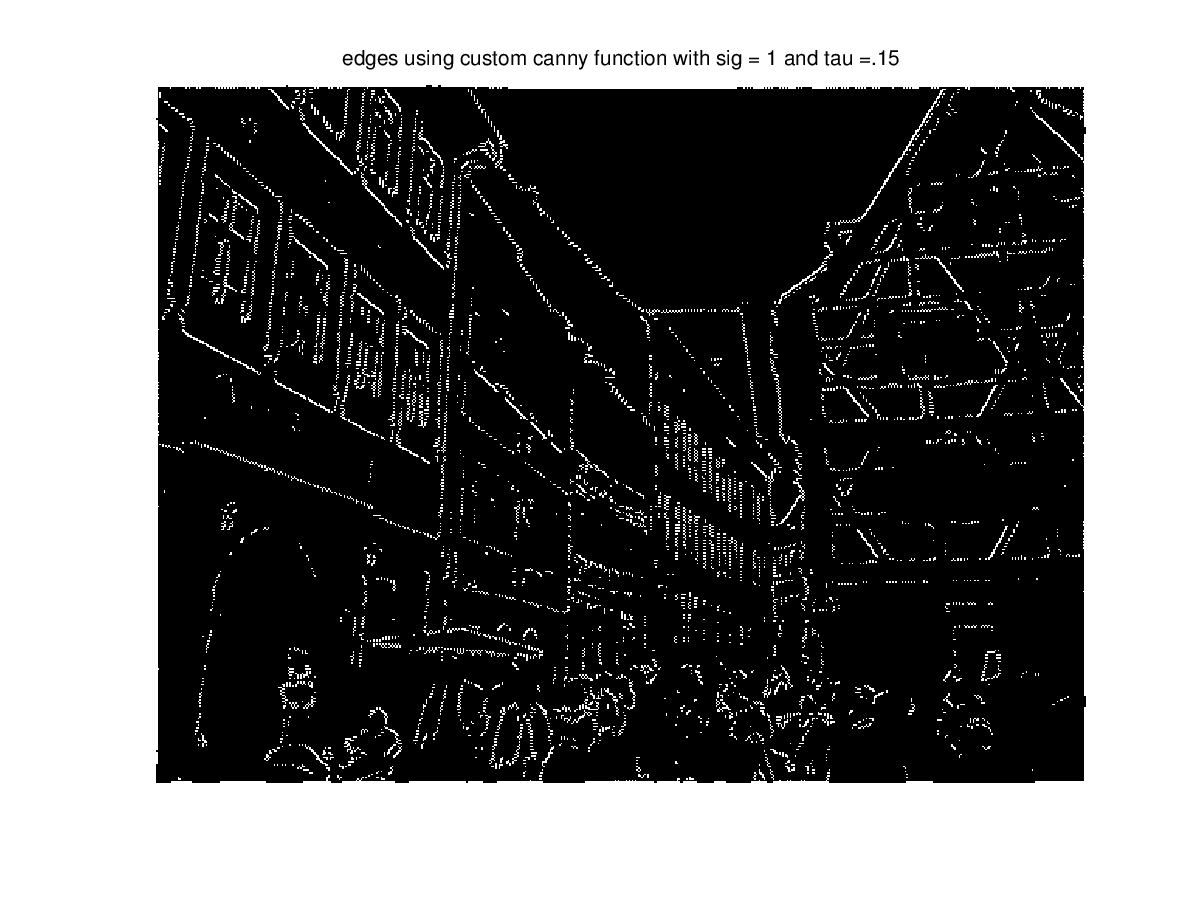
\includegraphics[width=\linewidth]{Q5/partD2.png}
	\end{figure}
	The results of the matlab function are much better than the custom made one. The difference in performance can be attributed to the lack of hysteresis thresholding and border artifacts. The border artifacts mess up the thresholding, since they have a much higher intensity, while the lack of hysteresis thresholding makes the edges look choppy.
	\newpage
	\section{Problem 6}
	\subsection{Apply the line hough transform to city.jpg}
	
	\begin{figure}[H]
		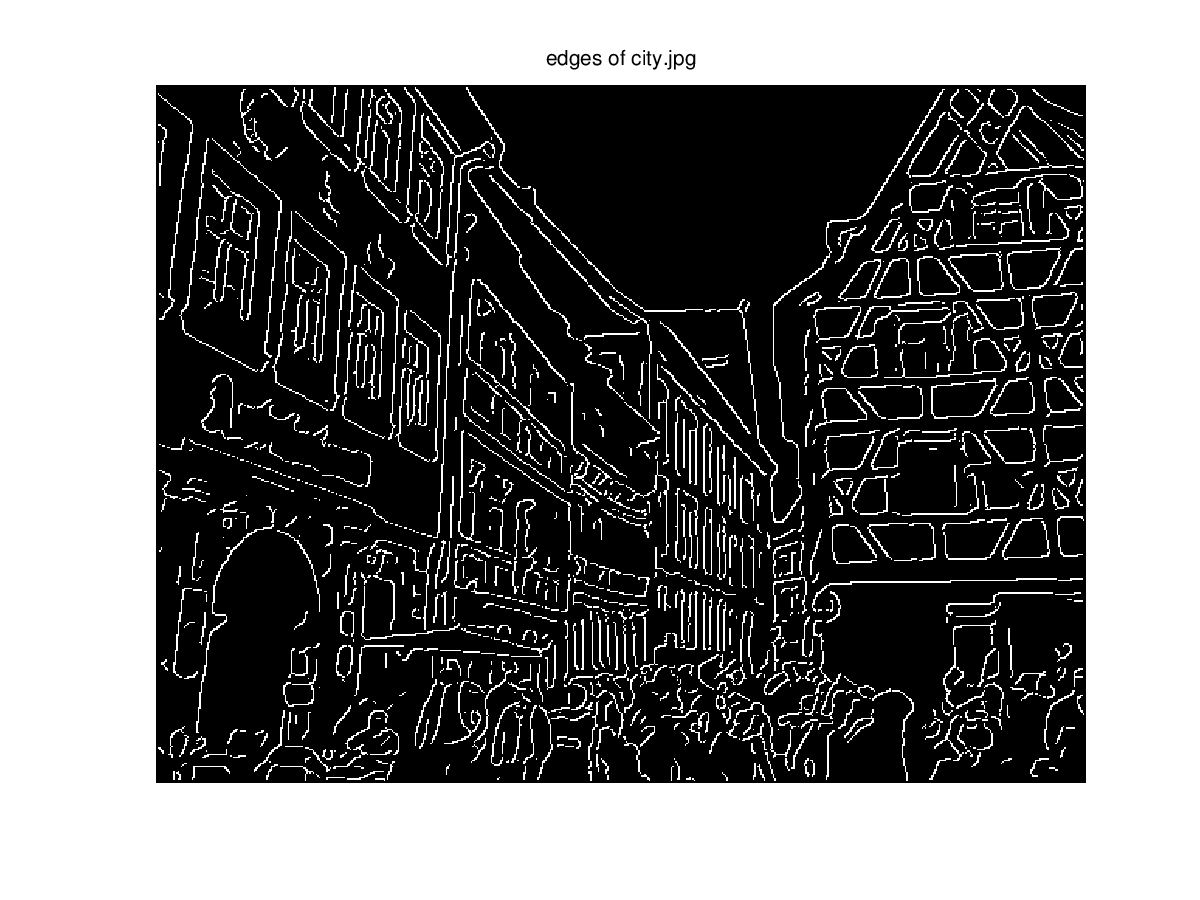
\includegraphics[width=\linewidth]{Q6/partA3.png}
	\end{figure}
	
	\begin{figure}[H]
		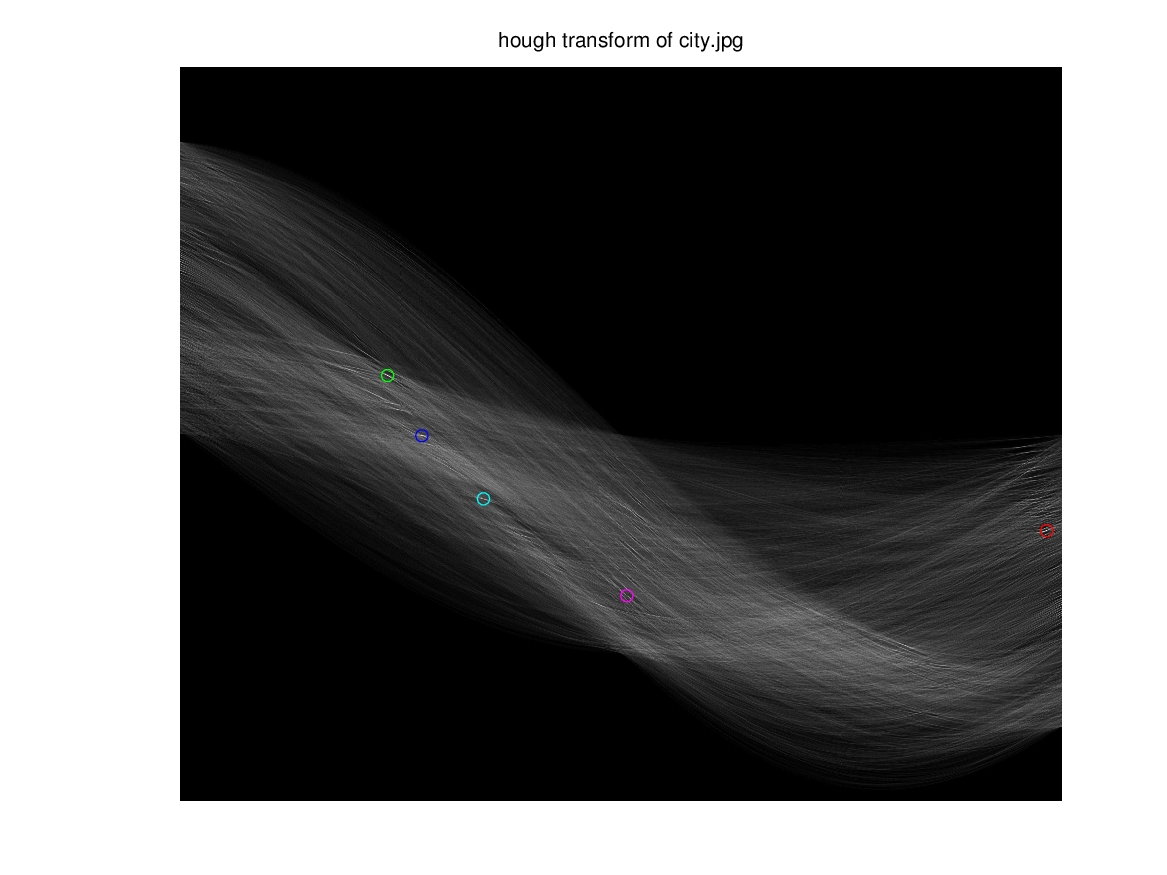
\includegraphics[width=\linewidth]{Q6/partA1.png}
	\end{figure}
	\begin{figure}[H]
		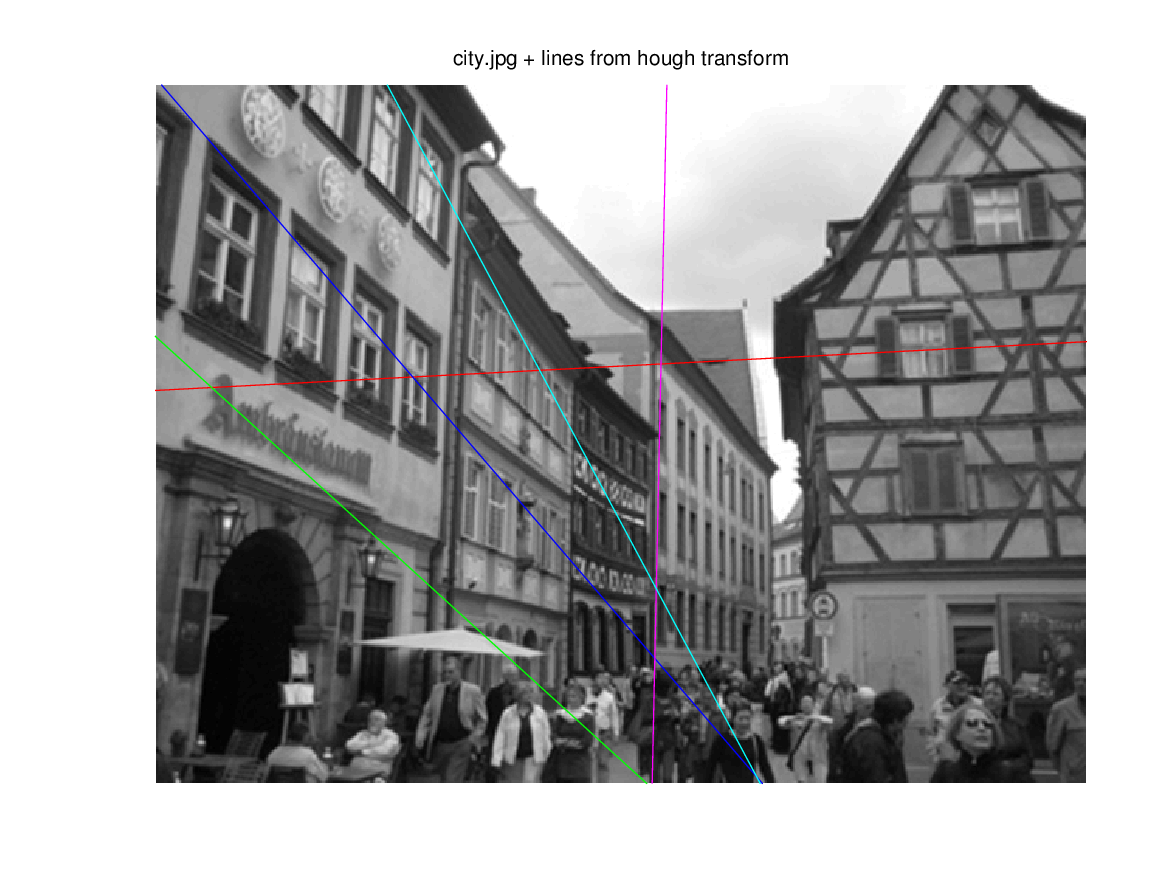
\includegraphics[width=\linewidth]{Q6/partA2.png}
	\end{figure}
	
	\newpage
	\subsection{Apply the circle hough transform to quarters.bmp}
	
	\begin{figure}[H]
		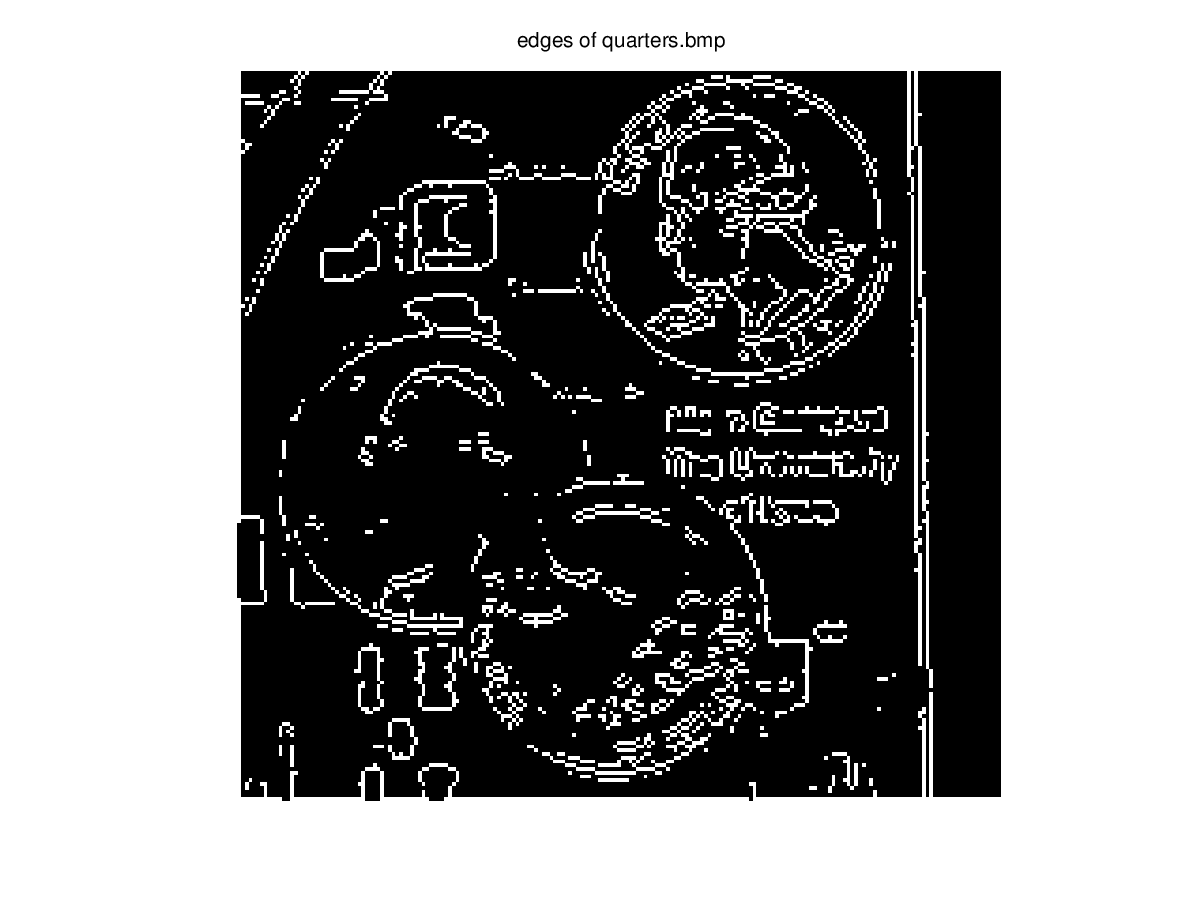
\includegraphics[width=\linewidth]{Q6/partB1.png}
	\end{figure}
	\begin{figure}[H]
		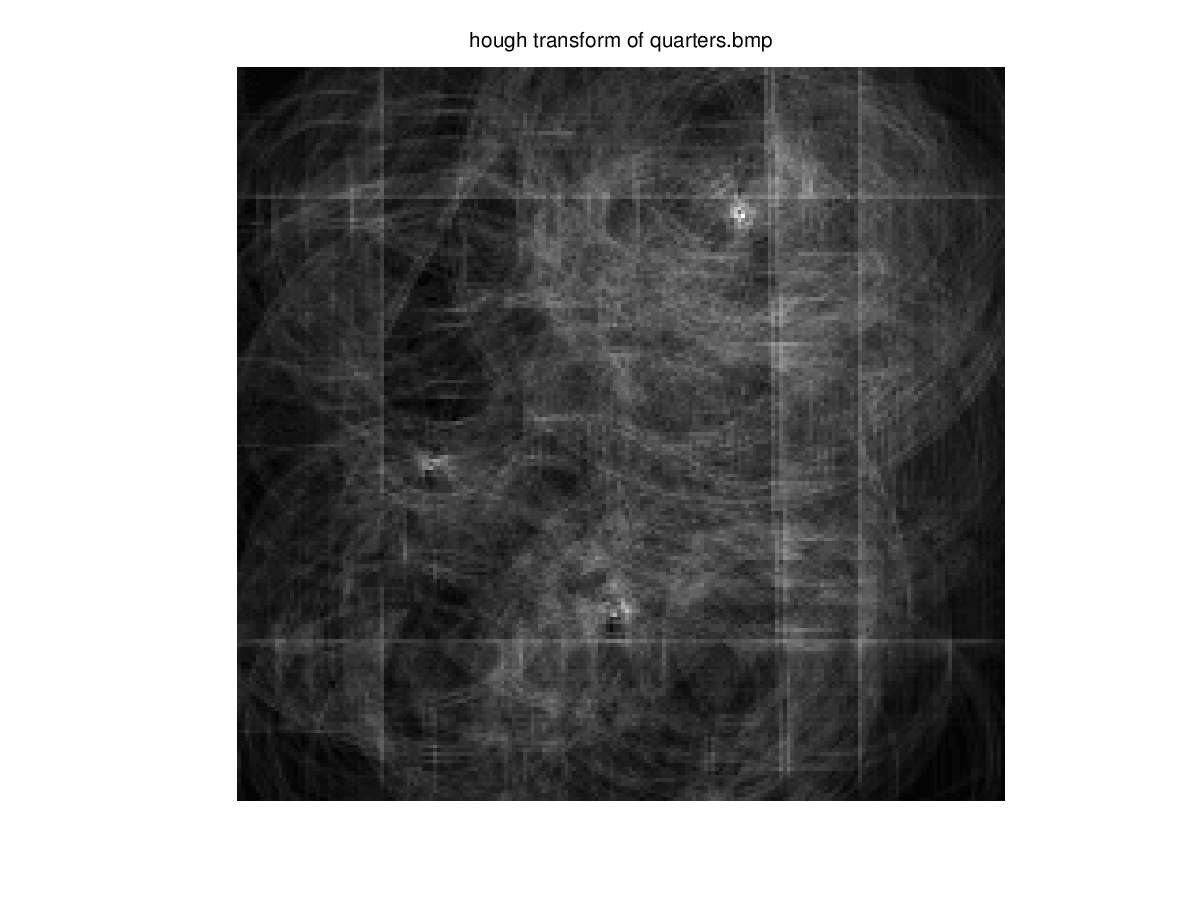
\includegraphics[width=\linewidth]{Q6/partB2.png}
	\end{figure}
	\begin{figure}[H]
		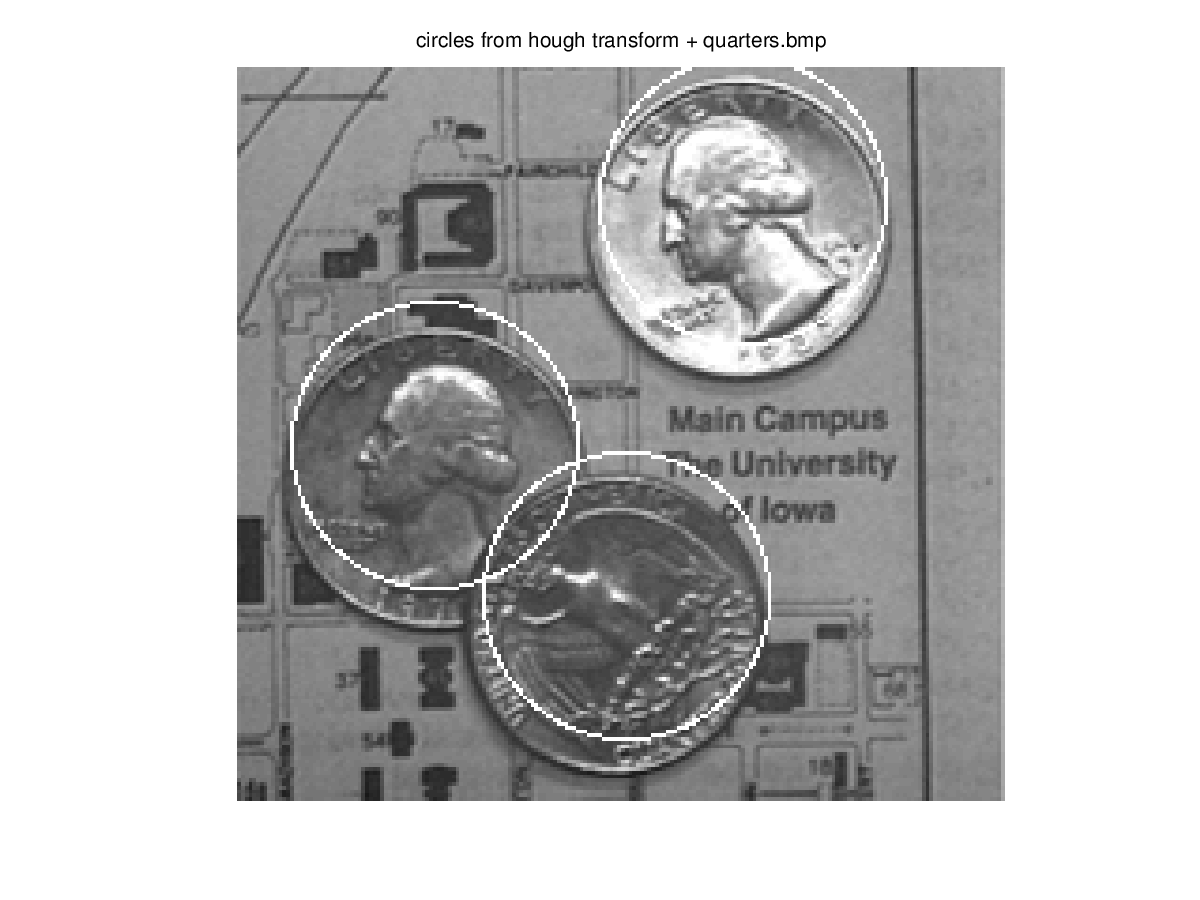
\includegraphics[width=\linewidth]{Q6/partB3.png}
	\end{figure}
	
	\newpage
	\section{Code}
	
	Part 5.A
	\lstinputlisting[language=Octave]{Q5/gradkernel.m}
	\newpage
	
	Part 5.B
	\lstinputlisting[language=Octave]{Q5/canny.m}
	\newpage
	
	Part 5.C
	\lstinputlisting[language=Octave]{Q5/partC.m}
	\newpage
	
	Part 5.D
	\lstinputlisting[language=Octave]{Q5/partD.m}
	\newpage
	
	Utility Code
	\lstinputlisting[language=Octave]{Q5/normalizeImage.m}
	\newpage
	
	Part 5.A
	\lstinputlisting[language=Octave]{Q6/partA.m}
	\newpage
	
	Part 5.B
	\lstinputlisting[language=Octave]{Q6/houghCircle.m}
	\newpage
	
	\lstinputlisting[language=Octave]{Q6/partB.m}
	\newpage
	
	
	
	
	
	
	
	
\end{document}
